\documentclass[../thesis.tex]{subfiles}
\section{Contagion on the Model}

Now that the groundwork has been layed down, we can focus on the object of our inquiry: demand shocks and price contagions. As equation (\ref{local_p_comp}) shows, price contagion depends, via $P(\matr{Y})$, on the matrix $(2\matr{I} + \matr{G})^{-1}$ which we can define as the ``bargaining power'' matrix, since it allocates the excess revenues, $\Delta_t$, among providers in the network. For example, in the case of a positive demand shock and an increase in the local price of electricity of a given node, the excess demand will be partially absorbed by all other nodes in the network which, in turn, causes a contagion of local price hikes. Hence, the spread of the price hikes depends on the bargaining power of nodes in the matrix. Sticking with our example, if $X_{i, t}$ increases suddenly, $\Delta^{(i, j)}_t$ increases, and the cross-border prices across the network increase by
\begin{equation*}
    (2\matr{I} + \matr{G})^{-1}_{(k, l), (i, j)}
\end{equation*}

This implies that a provider with a stronger bargaining position reacts more strongly to price changes, captures higher revenue, which leads to higher prices in the local market. Intuitively it also follows that a denser network, which results in a more equal distribution of bargaining power, leads to lower revenues for providers and lower price hikes. To formalize this, consider the entry $(i, j)$ in $P(\Y_t)$,

\begin{equation*}
    P^{(i, j)}_t = \frac{\sum_{(l, m) \in E} \Delta^{(l, m)}_t \cdot (2\matr{I} + \matr{G})^{-1}_{(i, j), (l, m)}}{Y^{(i, j)}_t},
\end{equation*}

where $\sum_{(l, m) \in E}$ is a summation over the row $(i, j)$ of $(2\matr{I} + \matr{G})^{-1}$. Now assume there is some demand shock in a node $k$. We would like to understand the effect this has on prices today, $P^{(i, j)}_t$, and tomorrow, $P^{(i, j)}_{t+1}$. To do so we can first note that the current traded quantity between the two nodes $i$ and $j$, $Y^{(i, j)}_t$, is not affected by a change in $X_{k, t}$ since it will only affect current prices and future quantities between $i$ and $j$ ($X_{k, t} \rightarrow P^{(i, j)}_{t} \rightarrow p_{i, t} \rightarrow X_{i, t+1}$), hence $\partial Y^{(i, j)}_t / \partial X_{k, t} = 0$. This is of course not true for $Y^{(i, j)}_{t+1}$. Now,

\begin{equation}
    \begin{split}
        \frac{P^{(i, j)}_{t}}{\partial X_{k, t}} &= \frac{1}{Y^{(i, j)}_t} \left( p_{k, t} \cdot \sum_{(k, m) \in E} (2\matr{I} + \matr{G})^{-1}_{(i, j), (k, m)} - p_{k, t} \cdot \sum_{(l, k) \in E} (2\matr{I} + \matr{G})^{-1}_{(i, j), (l, k)} \right) \\
        &= \frac{p_{k, t}}{Y^{(i, j)}_t} \underbrace{\left(\sum_{(k, m) \in E} (2\matr{I} + \matr{G})^{-1}_{(i, j), (k, m)} -  \sum_{(l, k) \in E} (2\matr{I} + \matr{G})^{-1}_{(i, j), (l, k)} \right)}_{\text{influence of $k$ on the network}}
    \end{split}
\end{equation}

\begin{figure}[!ht]
    \centering
    % First row
    \begin{subfigure}[t]{.4\textwidth}
        \centering
        \includegraphics[width=\linewidth]{\bargpath/line.pdf}
        \caption{On a sequential graph} \label{fig:linepower}
    \end{subfigure}
    \hfill
    \begin{subfigure}[t]{.4\textwidth}
        \centering
        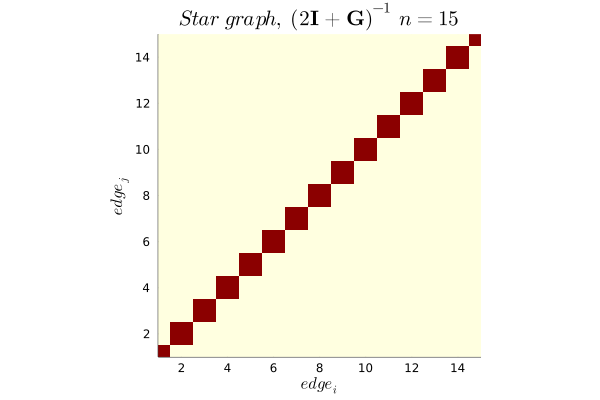
\includegraphics[width=\linewidth]{\bargpath/star.pdf}
        \caption{On a star graph} \label{fig:starpower}
    \end{subfigure}


    \medskip

    % Second row
    \centering
    \begin{subfigure}[t]{.4\textwidth}
        \centering
        \includegraphics[width=\linewidth]{\bargpath/binarytree.pdf}
        \caption{On a binary tree} \label{fig:btreepower}
    \end{subfigure}
    \caption{Network influence} \label{fig:influence}
\end{figure}

This influence value gives a first order approximation of the effect on the network of a demand shock in a given node. To get a better understanding of the model's construction and forces it is useful to go through a few simple cases analytically.

\subsection{Examples}

\subfile{sections/examples/twoproviders.tex}
\subfile{sections/examples/star.tex}
\subfile{sections/examples/line.tex}

\subsubsection{Conclusion}

In Figure \ref{fig:influence} I plotted the influence of each node on different graphs that will be used in the simulation. It is wise to stop here with the analytical work given the complex behavior of $P^{(i, j)}_{t + 1} / \partial X_{k, t}$, hence in the next section I will look at contagion by means of simulation.

\subsection{Contagion simulation}

To understand how price hikes propagate through the network in time, let's compare what happens simulating an equivalent demand shock in the central node of a sequential graph and a star graph (Figure \ref{fig:transshockcen}). In particular in the two figures I plot the evolution of prices and electricity supply after a 10 period shock (shaded area). This exercise brings with it a few interesting insights. First, it shows how relevant the network structure is for propagation. In the star graph, the price hike not only is much more pronounced but it is also sustained for longer. Furthermore, the network structure allows for the price increase to be much more persistent, lasting, in the case of the star graph, almost twice as much as the demand shock. This self-fulfilling behavior persists until electricity production is high enough to push prices back down to their equilibrium levels. Importantly, this has to happen throughout the network, instead of simply in the central node.

\begin{figure}[!ht]
    \begin{subfigure}{0.45\textwidth}
        \centering
        \includegraphics[width = \textwidth]{\plotpath/central/line/pricesupply.pdf}
        \caption{Sequential graph}
    \end{subfigure}
    \hfill
    \begin{subfigure}{0.45\textwidth}
        \centering
        \includegraphics[width = \textwidth]{\plotpath/central/star/pricesupply.pdf}
        \caption{Star graph}
    \end{subfigure}
    \caption{Prices and supply with a transient shock in a central node} \label{fig:transshockcen}
\end{figure}

Another interesting variable to track during the shock is the excess demand in each node $X_{i, t}$. In the current simulation the ``expected'' excess demand has to be fulfilled, namely $\sum_i \E_{i, t-1}\left[X_{i, t}\right] = 0$, since its stems from the optimization problem of the provider. Nevertheless, the realized excess demand might be positive, $\sum_i X_{i, t} > 0$. In this case a ``blackout'' occurs, namely prices fail to induce enough electricity supply. Figure (\ref{fig:profittransshockcen}) shows the evolution of $X_{i, t}$ and $\sum_i X_{i, t} > 0$. This figure, once again, delivers both a trivial and a more surprising insight. Trivially, the shock in excess demand causes in both graphs a ``blackout'', which is more pronounced in the case of the sequential graph due to a weaker price transmission and a weaker supply adjustment. Surprisingly, the shock brings in the long term a long period of oscillating production which leads to periodic ``blackouts''. This phenomenon arises due to the ``naive'' view that agents have of the pricing mechanism process. In the star graph, the price hike propagates throughout the network immediately, since all nodes are linked to the central node. This causes production to increase in all peripheral nodes, which in turn generates a excess electricity supply. This overshooting creates strong downward pressure on prices, via cross-border prices and expectations of providers, which keeps supply artificially low for a sustained time period. A smaller overshoot, as in the case of the sequential graph, causes a bigger immediate ``blackout'' but a smaller persistence of low prices in time.

\begin{figure}[!ht]
    \begin{subfigure}{0.45\textwidth}
        \centering
        \includegraphics[width = \textwidth]{\plotpath/central/line/demand.pdf}
        \caption{Sequential graph}
    \end{subfigure}
    \hfill
    \begin{subfigure}{0.45\textwidth}
        \centering
        \includegraphics[width = \textwidth]{\plotpath/central/star/demand.pdf}
        \caption{Star graph}
    \end{subfigure}
    \caption{Excess demand $X_{i, t}$ with a transient shock in the central node} \label{fig:profittransshockcen}
\end{figure}